\documentclass[hidelinks]{article}

%All lines down is for fontawesome icons-----------------------
% Needed to use \ifxetex-\else-\fi statement
\usepackage{ifxetex}
% Needed to use \if-\then-\else statement
\usepackage{xifthen}
% Needed to use a toolbox of programming tools
\usepackage{etoolbox}
% Needed to change line spacing in specific environment
\usepackage{setspace}
% Needed to manage fonts
\ifxetex
  \usepackage[quiet]{fontspec}
  % To support LaTeX quoting style
  \defaultfontfeatures{Ligatures=TeX}
\else
  \usepackage[T1]{fontenc}
  % Replace by the encoding you are using
  \usepackage[utf8]{inputenc}
\fi
\usepackage{fontawesome}
%-----------------------------------------------------------

\usepackage{tabto} %tabCommand
\usepackage{titlesec}
\usepackage[utf8]{inputenc}
\usepackage{titling}
\usepackage{xcolor}
\usepackage{color}
\usepackage{smartdiagram}
\usepackage[margin=0.6in]{geometry}
\usepackage{hyperref}
\usepackage{tikz}
\usetikzlibrary{calc,positioning,backgrounds,matrix}
\usepackage[openbib]{currvita}
\usepackage[absolute]{textpos}
\usepackage{xhfill}
\usepackage{amssymb} %checkbox
\usepackage{tikz}
\usetikzlibrary{trees}
\usepackage{setspace} % control space bet. lines%

\definecolor{dimgray}{rgb}{0.41, 0.41, 0.41}
\definecolor{blue}{RGB}{0,51,128}
\hypersetup{
    colorlinks=true,
    linkcolor=blue,
    filecolor=magenta,      
    urlcolor=blue,
}


% Title name
\renewcommand{\maketitle}{
\begin{center}
\Huge\bfseries
\color{dimgray}\thetitle
\vspace{0em}
\Large\bfseries
\vspace{0em}
\color{blue}\theauthor
{}
\end{center}
\vspace{-1em}
\xhrulefill{dimgray}{3pt}

}


\usepackage{sectsty}
\sectionfont{\color{blue}}
\renewcommand{\thesubsubsection}

\titleformat{\subsubsection}
{\small}
{}
{0em} 
{}
  
\titleformat{\section}
{\small\bfseries\uppercase}
{}
{-5px} 
{}

\smartdiagramset{
      bubble center node font = \Large,
      bubble node font = \bfseries\normalsize,
      bubble center node size =2.84 cm,
      bubble node size =2.5cm,
    }

\color{black}
\begin{document}
%\begin{textblock}{width}[xt,yt](X,Y)
\begin{textblock}{3.3}(.6,0)

\section*{Personal Info.}\vspace{-4pt}
\textcolor{blue}{\LARGE\faMobile}\space\space +201151280909\\[3pt]
\textcolor{blue}{\large\faHome}\space\space10 St. Ibrahim Baher Zaghlol, Manial, Cairo, Egypt \\[3pt]
\href{mailto: habiba.hamad97@eng-st.cu.edu.eg}{\textcolor{blue}{\faEnvelope}}\space\space\space{\textcolor{black}{habiba.hamad97@eng-st.cu.edu.eg}}

\vspace{-4pt}

%Another Way using fontawesome :D -----------------
%{\Large\faMobile}\space\space\space +201151280909 \\[3pt]
%{\large\faHome} \space\space  10 St. Ibrahim Baher Zaghlol, Manial, Cairo, Egypt \\[3pt]
%\faEnvelope\space\space\space\href{mailto: habiba.hamad97@eng-st.cu.edu.eg}{ habiba.hamad97@eng-st.cu.edu.eg}


\section*{Work Profiles}\vspace{-4pt}

\includegraphics[scale=0.0175]{github.png}\space\space\href{https://github.com/habiba1997}{/habiba1997} \\[4pt]
\href{https://www.linkedin.com/in/habiba-ahmed-563399127}{\faLinkedin\space\space/Habiba Ahmed} \\[4pt]

\includegraphics[scale=0.015]{hackerrank.png}\space\space\href{https://www.hackerrank.com/habiba_hamad97}{/habiba\_hamad97}

\vspace{-4pt}

\section*{Programistic Skills}\vspace{-4pt}

   \smartdiagram[bubble diagram]{Java,C++,Python,Image \\ Processing,Matlab,C\# , Machine \\ Learning,\LaTeX} 
    
 \vspace{-10pt}
 
\section*{Full Stack Web Development}\vspace{-2pt}
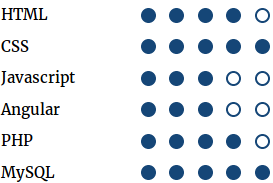
\includegraphics[scale=0.65]{Web.png}
\section*{Interpersonal Skills}\vspace{-2pt}

\makebox[0pt][l]\tab{\color{blue}\hspace{0.1em}$\checkmark$}	Leadership 

\makebox[0pt]\tab{\color{blue}\hspace{-1.5em}$\checkmark$}	Time Management 

\makebox[0pt]\tab{\color{blue}\hspace{-1.5em}$\checkmark$}	Assiduous \& Organized

\makebox[0pt]\tab{\color{blue}\hspace{-1.5em}$\checkmark$}	Hardworker
 
\makebox[0pt]\tab{\color{blue}\hspace{-1.5em}$\checkmark$}	Team Management 
 
\makebox[0pt]\tab{\color{blue}\hspace{-1.5em}$\checkmark$}	Strong work ethics

\section*{Languages}

\includegraphics[scale=0.55]{languages2.png}
\end{textblock}

\begin{textblock}{9.4}(5.9,.1)

\title{Habiba Ahmed\\}
\author{System and Biomedical Engineering Student}
\maketitle
\vspace{-.75em}

\section*{Education}
\vspace{-4pt}
\begin{cvlist}{}
\item[2015--2020] Systems and Biomedical Engineering, Cairo University \\* (GPA: 3.78)
\item[2013--2015] Oruba International High School (American Diploma)
\end{cvlist}
\section*{College Related Courses}\vspace{-4pt}
%Content: Static Arrays, Dynamic Arrays, Struct, Stacks, Linked Lists, Queues, Priority Queues, Binary Search Trees, Sets, Maps, Heaps, and finally Hash Tables.
\begin{cvlist}{\vspace{-10pt}}
\item[2/2018--6/2018] Algorithm and Data Structure Using C++ Language
\item[2/2018--6/2018] Object Oriented Programing Using Java
\item[10/2018--1/2019] Databases and File Structure Using MySQL
\item[10/2018--1/2019] Probability and Statistics

\end{cvlist} 


\section*{Competitions} \vspace{-4pt}
\begin{cvlist}{}
\item[1/08/2018 -- 14/10/2018] Hospital System Innovation Competition, CUFE
\item[19/10/2018 -- 20/10/2018] IEEEXtreme Programming Competition

\end{cvlist}

\section*{Experience}\vspace{-4pt}
\begin{cvlist}{} 
\item[07/2017--06/2018] Vice President @ Hand In Hand \\ Charity Student Activity
\item[09/2017--05/2018] Head Public Relation @ BEAT \\ Biomedical Engineering Awareness and Technology
\item[06/2017--09/2017] Fundrasing Member @ International Student Conference
\end{cvlist}

\section*{Personal Projects}\vspace{-4pt}
\subsubsection{HNA hospital (Competition Project)}
A smart registration, data access and storage hospital system 

\subsubsection{Medium (Web Development Project)}
A simulation for medium.com website

\subsubsection{Immature Babies Nursery}
A baby incubator simulation using arduino, Color Sensor, Thermistor, and Turbine Flow Sensor

\subsubsection{Question and Answer Game}
A python GUI game where a player answer various questions related to his choosen subject

\section*{Certifications}\vspace{-4pt}
\begin{cvlist}{}
\item[9/2018--Present] Cloud Introduction \\ Certification authority IBM
\item[2/2017--Present] Project Management: The Basics for Success\\Certification authority Coursera

\end{cvlist}

\end{textblock}


\end{document}
